\scanpage{39}
\mspage{\textcircled{20}}
locates \inserted{the} $u(\widetilde a_i^\omega)$, already follows from that of $\zeta$, which locates \inserted{the} $u(d_i^\omega)$,
\figure{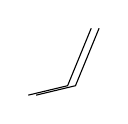
\begin{tikzpicture}[baseline=0pt]\draw (0,0)--(.5,.12)--(.8,.85);\draw (.1,0)--(.6,.12)--(.9,.85);\end{tikzpicture}}
The graphs $\overline{\underline{\mathrm{I}}}$ to $\overline{\underline{\mathrm{VII}}}$ give rise to the diagram of inclusions
\diagram{\begin{tikzcd}[ampersand replacement=\&,column sep=2em,row sep=2.8em,execute at end picture={\draw ([xshift=-4mm,yshift=5mm]\tikzcdmatrixname-2-1.north west) rectangle ([xshift=5mm,yshift=-4mm]\tikzcdmatrixname-3-3.south east);}]
\&\&\overline{\underline{\mathrm{III}}}\arrow[dl,hook]\arrow[dr,hook]\&\&\\
\overline{\underline{\mathrm{I}}}\arrow[r,hook]\arrow[dr,hook]\&\overline{\underline{\mathrm{II}}}\arrow[dr,hook]\arrow[r,draw=none,"\deleted{\leftrightarrow}"]\&\phantom{\overline{\underline{\mathrm{II}}}}\&\overline{\underline{\mathrm{IV}}}\arrow[dl,hook]\&\mathrm{V}\arrow[l,hook]\\
\&\overline{\underline{\mathrm{VII}}}\arrow[r,hook]\&\overline{\underline{\mathrm{VI}}}\&\&
\end{tikzcd}}\quad(68)

Without calculation, I can already predict that giving an automorphism of $\overline{\underline{\mathrm{VII}}}$ fixing the vertices and commuting with $G_J$, is equivalent to giving the quantities
\[
(69)\qquad (\uline{\lambda},\beta',\uline{\zeta'})\in\widehat\Pi_{0,3}\times\widehat\Pi_{0,3}\times\widehat\Pi_{0,3}
\]
related by \deleted{\unsure{the}}the equations \deleted{(63) here}
\[
(70)\qquad\left\{\begin{aligned}
\beta'&=\alpha'\sigma_\infty(\lambda)\\
\beta'\sigma_\infty(\beta')&=1
\end{aligned}\right.\qquad
\begin{gathered}
\text{where}\quad\alpha'=\zeta'\rho^{\deleted{\unsure{-1}}}(\zeta')^{-1}\\
\text{i.e.}\quad\alpha'\sigma_\infty(\lambda)\sigma_\infty(\alpha')\lambda=1
\end{gathered}
\]
\margin{\figure{
\begin{tikzpicture}\node[align=center] at (0,.6) {so $\beta'$\\unnecessary!};\draw (-.8,.6)..controls (-.9,-.1) and (-.2,-.3)..(0,-.6)..controls (.05,-.1) and (.85,-.2)..(.9,.35);\end{tikzpicture}}}
(just as \inserted{in the case where} $\overline{\underline{\mathrm{II}}}$ is defined by \deleted{$(\lambda,\eta,\alpha')$},
\deleted{related by}
\[
(69')\qquad(\uline{\lambda},\uline{\eta},\alpha')\in\widehat\Pi_{0,3}\times\widehat\Pi_{0,3}\times\widehat\Pi_{0,3}
\]
with \unsure{the|the} equations
\[
(70')\qquad\left\{\begin{aligned}
\beta'&=\alpha'\sigma_\infty(\lambda)\\
\alpha'\rho(\alpha')\rho^2(\alpha')&=1
\end{aligned}\right.\qquad\text{where}\quad\beta'=\eta\sigma_\infty(\eta)^{-1}
\]
\margin{so $\alpha'$ unnecessary!}
\margin{38}
